% De espacio de estados a función de transferencia: G(s)=C(sI-A)^{-1}B+D
\documentclass[border=6pt]{standalone}
\usepackage{amsmath}
\usepackage{tikz}
\usetikzlibrary{arrows.meta, calc}
\begin{document}
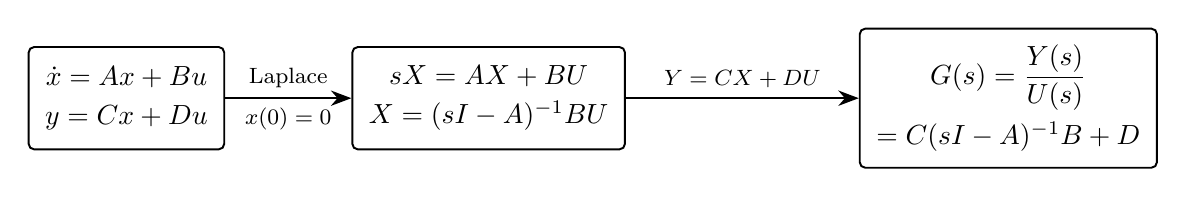
\begin{tikzpicture}[
  >={Stealth[length=2.6mm]}, line width=0.7pt,
  caja/.style={draw, rounded corners=2pt, align=center,
               minimum height=1.3cm, inner sep=6pt}]

  \node[caja] (ss) at (0,0)
    {$\dot{x}=Ax+Bu$\\[2pt]$y=Cx+Du$};
  \node[caja] (res) at (4.6,0)
    {$sX=AX+BU$\\[2pt]$X=(sI-A)^{-1}BU$};
  \node[caja] (ft) at (11.2,0)
    {$G(s)=\dfrac{Y(s)}{U(s)}$\\[3pt]$=C(sI-A)^{-1}B+D$};

  \draw[->] (ss) -- (res) node[midway, above]{\footnotesize Laplace}
                          node[midway, below]{\footnotesize $x(0)=0$};
  \draw[->] (res) -- (ft) node[midway, above]{\footnotesize $Y=CX+DU$};
\end{tikzpicture}
\end{document}
